\documentclass[tikz]{standalone}

\usepackage{ifthen}
\usetikzlibrary{calc}

\newcommand{\surround}[2]{\draw[rounded corners] ($#2-(1em,1em)$) rectangle ($#2 + (#1,#1) + (1em,1em)$);}
\newcommand{\drawpointgrid}{
\foreach \x in {0,1,...,5}
  \foreach \y in {0,1,...,5}
  {
  \node[circle, inner sep=0.05em, fill] at (\x,\y) {};
  }

\foreach \x in {0,2,4}
  \foreach \y in {0,2,4}
  {
  \ifthenelse{\x=0 \AND \y=0}{}{
  \surround{1}{(\x,\y)}
  }
  }
  
\draw[rounded corners] ($(0,1) + (-1em,-1em)$) -- ($(0,1) + (-1em,1em)$) --
				       ($(1,1) + (1em,1em)$) -- ($(1,0) + (1em,-1em)$) --
				       ($(1,0) + (-1em,-1em)$) -- ($(1,1) + (-1em,-1em)$) -- cycle;

}

\begin{document}

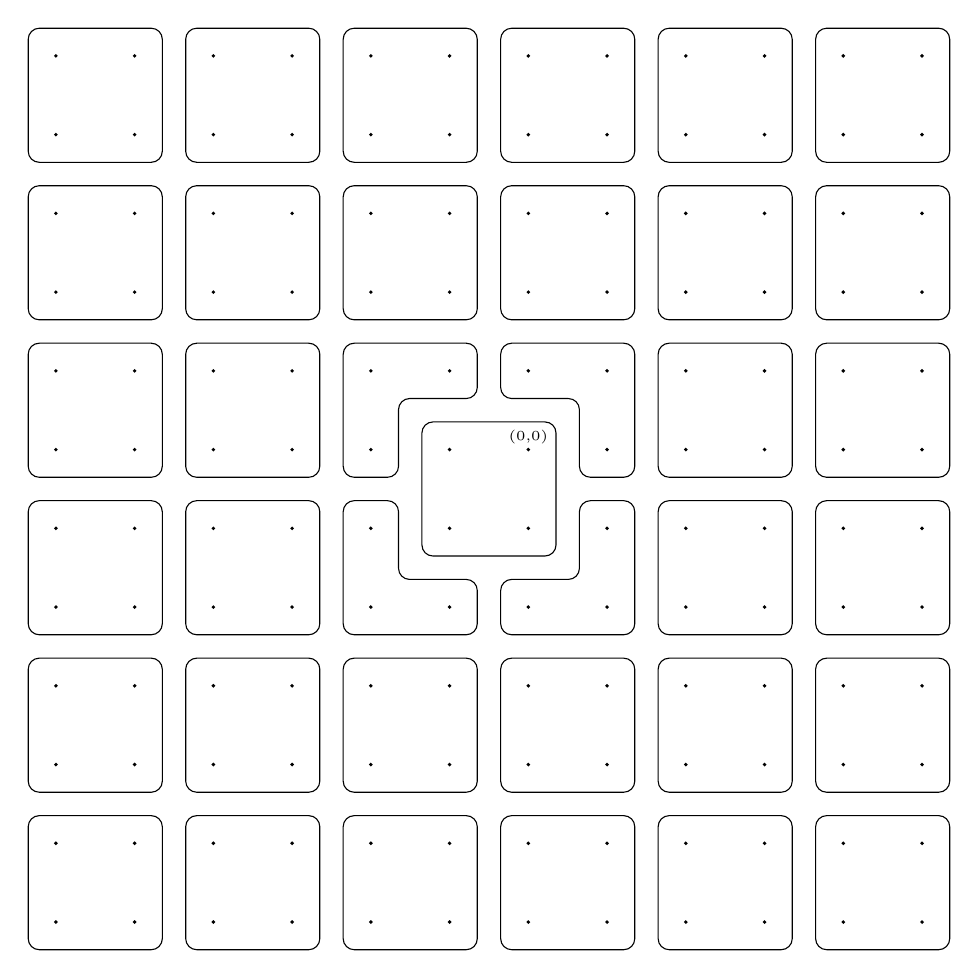
\begin{tikzpicture}
\drawpointgrid
\begin{scope}[yscale=-1,xscale=1,yshift=1cm]
	\drawpointgrid
\end{scope}
\begin{scope}[yscale=-1,xscale=-1,xshift=1cm, yshift=1cm]
	\drawpointgrid
\end{scope}
\begin{scope}[yscale=1,xscale=-1,xshift=1cm]
	\drawpointgrid
\end{scope}

\surround{1}{(-1,-1)}

\node[label={[label distance=-.5em]\tiny (0,0)}] at (0,0) {};

\end{tikzpicture}


\end{document}
